\section{Design}
The concept for the GeoLog originally came from Dr. Andrew D. Wickert, who came to Reykjavík University's Mechatronics class for 
help developing his design of a low cost and low power datalogger\cite{ALog-BottleLogger}. 
Dr. Wickert had two problems needed to be solved. Firstly to minimize the power consumption of the device he had already developed and secondly to have means of getting the data
back without having to travel through difficult terrain. Decision was made to help Dr. Wickert 
improve the latter with emphasis on making the system as modular as possible. This design assumes 
there is GSM/GPRS coverage in the area the system is deployed. It is also assumed that HTTP server has been set up for receiving data from GeoLog.
\begin{figure}
\centering
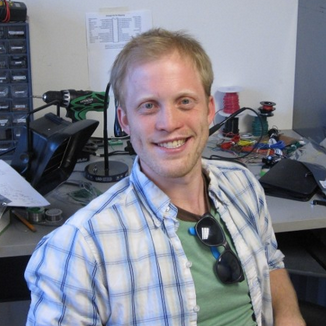
\includegraphics[width=0.4\linewidth]{graphics/andrewWickert}
\caption{Dr. Wickert\label{fig:andrewWickert}\cite{andrewWickert}}
\end{figure}
The GeoLog datalogger was designed in nine phases. Phases seven to eight are iterated
until the product is ready for deployment.
\begin{itemize}
    \item{Phase 1:} Initial brainstorming and high level design phase.
    \item{Phase 2:} Hardware selection phase, where hardware is selected and ordered.
    \item{Phase 3:} Software design phase, where the classes and interfaces is designed.
    \item{Phase 4:} Hardware hacking phase, trial and error in software writing for the
                    Wixels\cite{wixel} and the GSM/GPRS module\cite{SM5100B}.
    \item{Phase 5:} Building phase, where hardware is assembled.
    \item{Phase 6:} Software integration phase, all the software integrated to one.
    \item{Phase 7:} Field testing phase, testing of the system in real life environment.
    \item{Phase 8:} Fixing phase, fixing bugs found in the field testing phase.
    \item{Phase 9:} Deployment phase, system is functional and can be deployed. 
\end{itemize}
\subsection{Hardware}
\begin{figure}
\centering
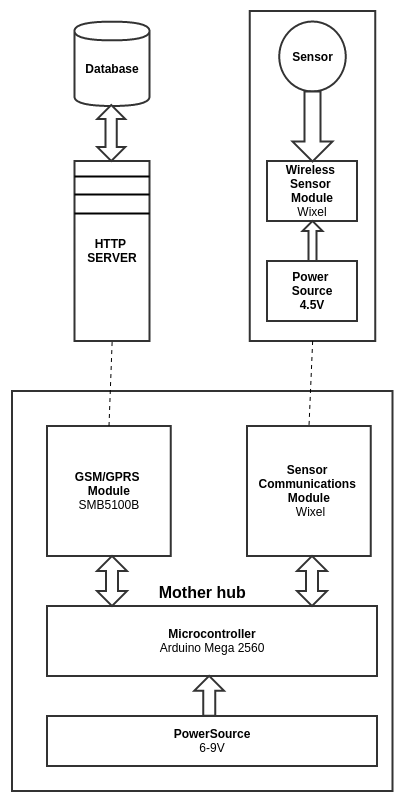
\includegraphics[width=0.5\linewidth]{graphics/HardwareMDD}
\caption{Hardware Module Design Diagram\label{fig:HardwareMDD}}
\end{figure}
\begin{figure}
\centering
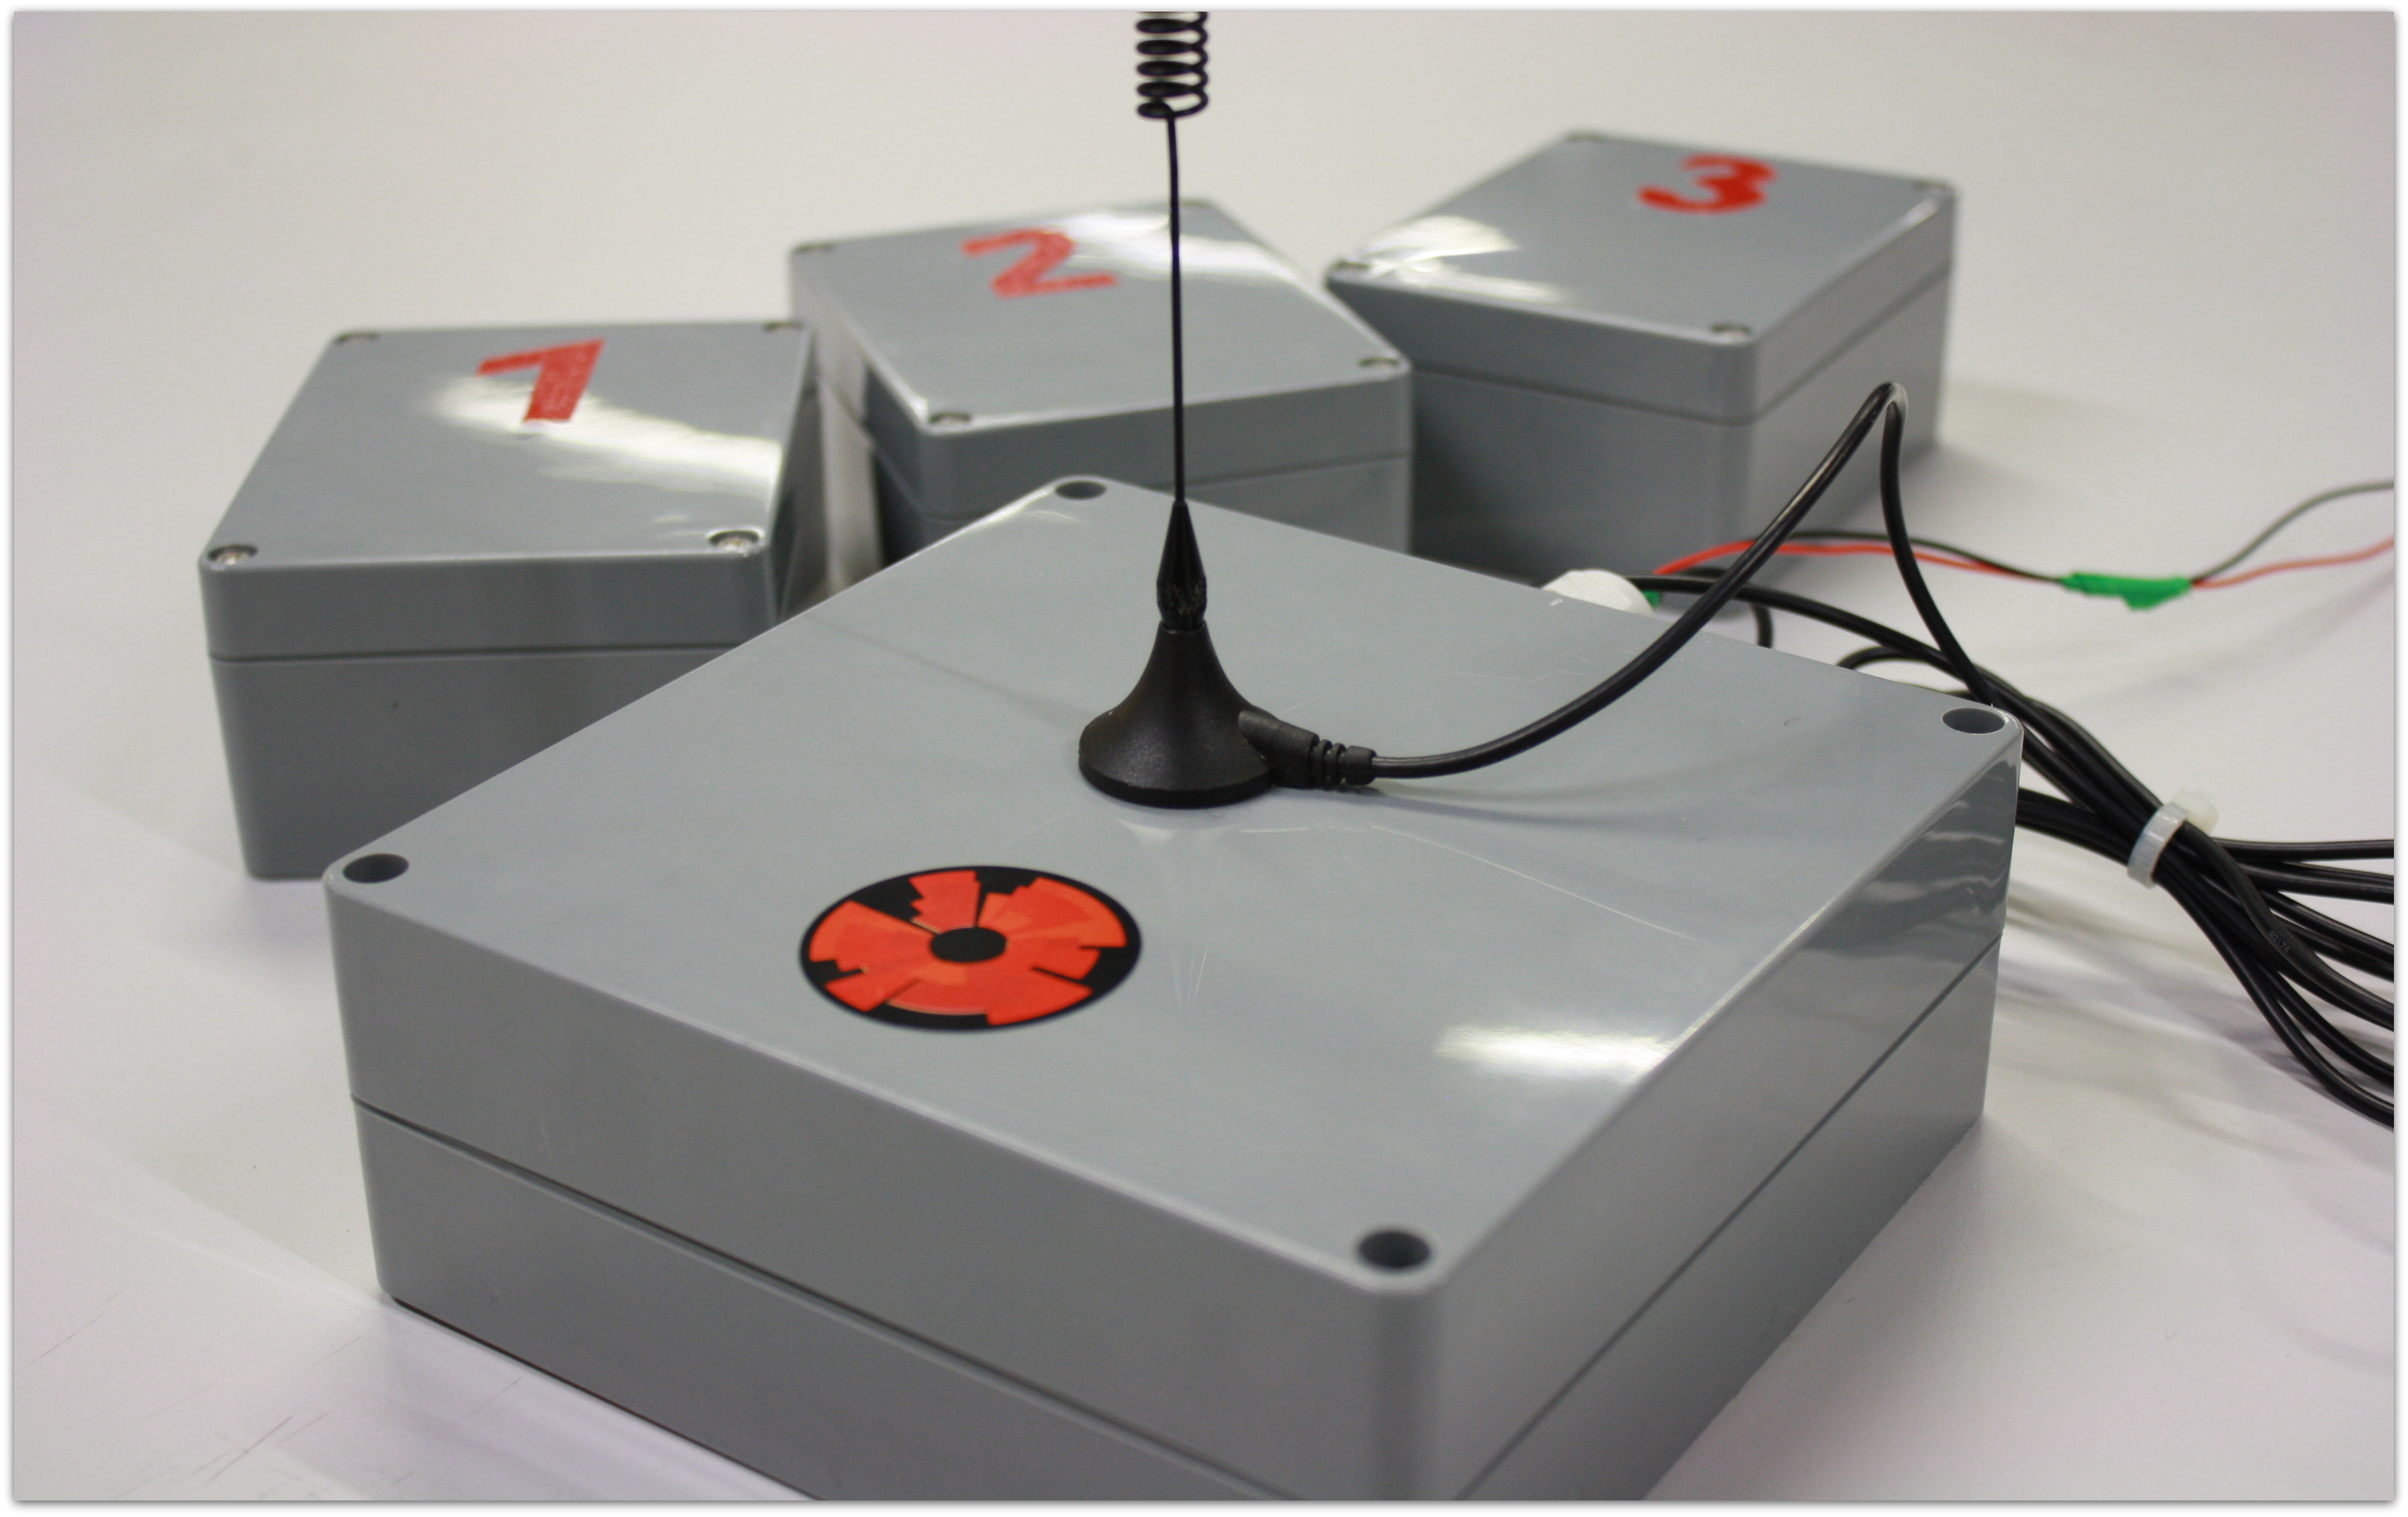
\includegraphics[width=0.8\linewidth]{graphics/Our_product}
\caption{Assembled product\label{fig:Our_product}}
\end{figure}
The hardware is divided into sensor modules and the mother hub. The sensor modules 
designed for this system were three wireless temperature sensors using Wixel\cite{wixel}
for means of communications. The mother hub consists of a Arduino Mega\cite{arduinoMega}
that communicates with the sensor modules with a Wixel, collects the data 
and sends it to a HTTP server via the GSM/GPRS module\cite{SM5100B}. See overview of the system in figure~\ref{fig:datalogging}. All modules are 
encased in a IP67\cite{ipRating} plastic enclosure for protection against difficult weather conditions.
Figure \ref{fig:HardwareMDD} shows hardware setup and figure \ref{fig:Our_product} shows the assembled 
product. 
\begin{figure}[H]
		\centering
        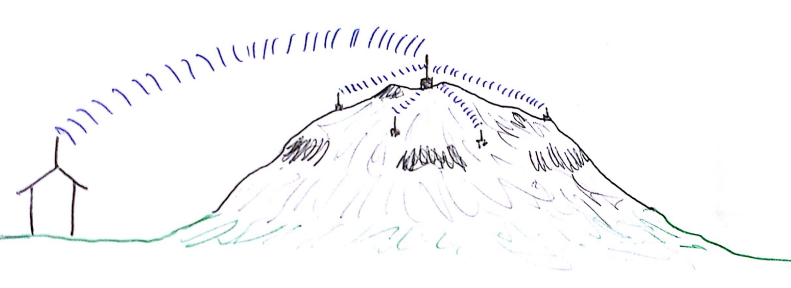
\includegraphics[height=6cm]{graphics/GeoLog.PNG}
        \caption{Demonstration drawing of wireless data collecting.}
        \label{fig:datalogging}
\end{figure}
\subsubsection{Sensor module}
The sensor module is based on Wixel\cite{wixel} which reads sensor value from it's
analog inputs when the mother hub calls for reading. To save energy the sensor module does
not send any data until it's id is called by the mother hub. The sensor module then 
gathers several readings from the sensor over a short period of time and sends back the 
average reading of the data collected. After sending the the data it falls back to suspend mode until the mother 
hub calls again for data. Electrical schematic diagram of the sensor module can
be seen in figure \ref{fig:sensormodule_schematic}.
\subsubsection{Mother hub}
The mother hub is based on Arduino Mega 2560\cite{arduinoMega} which can be switched out 
for Dr. Wickert's Bottle Logger\cite{ALog-BottleLogger}, a Wixel\cite{wixel} used for 
communicating with the wireless sensor modules and a SM5100B GSM/GPRS 
module\cite{SM5100B}. The mother hub gathers data from the Wireless sensor modules via 
the onboard Wixel by calling them by id and wait till corresponding sensor module answers
with newly gathered sensor data. The data gathered is then saved to its onboard EEPROM~\cite{EEPROM}.
At a preset time the data is sent to a HTTP server via GPRS~\cite{GPRS} where it can be processed 
by the researcher. Electrical schematic diagram of the mother hub can be seen in figure 
\ref{fig:motherhub_schematic}.
\subsection{Software}
\begin{figure}
\centering
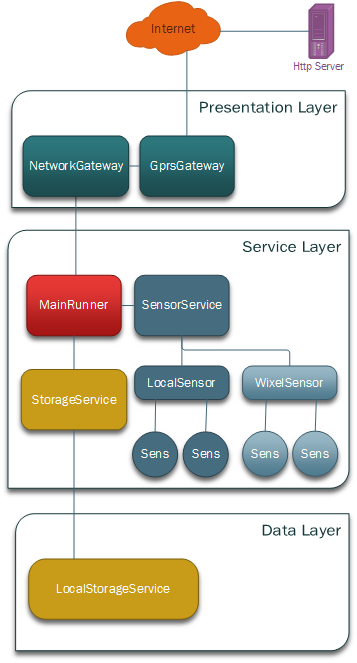
\includegraphics[width=0.6\linewidth]{graphics/Layering}
\caption{Layered Design Diagram of the system\label{fig:Layering}}
\end{figure}
When designing the software, modularity was the main interest and is better described as
a framework ready for different implementation. The design aims for making
it as versatile as possible and ready for implementation of new ways of communications, sensors and storage. This is done by building the software up of three interfaces the user needs to implement if for example another means of communications is needed. The system comes with two ways of communications to the outside world, a SMS gateway and a GPRS HTTP gateway. It also comes with one way of storing data, to the EEPROM and one way of communicating to wireless sensors. Figure \ref{fig:Layering} shows the layered design of the software. The GeoLog project is open source and anyone can contribute
to the project at \url{https://github.com/GeoLogTeam/geolog}.\\
To take a closer look in to the software and how the interfaces work see the class diagram
shown in figure \ref{fig:ClassDiagram}. Next sections will describe more thoroughly how each module works. All code is written in C++ except the HTTP server which is written in Python/Flask-Restful~\cite{Flask}.

\subsubsection{Sensor Service interface}
The sensor service is an interface the developer needs to implement for every new kind of
sensor module. The sensor service interface has three virtual functions that the developer
needs to implement by inheriting from the SensorService class.The functions that needs implementation are the following:
\begin{itemize}
    \item \textbf{int getSensorData(int sensorId)}
        \begin{itemize}
            \item Takes in the id of the sensor and returns the raw value.
        \end{itemize}
    \item \textbf{int sendDataToSensor(String data)}
        \begin{itemize}
            \item Takes in data to send to sensor and returns 0 for OK and -1 for error.
                  This could be used to remote calibrate sensor.
        \end{itemize}
    \item \textbf{int setDateTime(long DateTime)}
        \begin{itemize}
            \item Takes in UNIX date/time for setting the time on the sensor if needed.
        \end{itemize}
\end{itemize}
The sensor service now implemented is the WixelSensorService. This service communicates 
with the Wixel Sensor Modules, converts the raw data to a value of interest like 
temperature and finally parses the converted data to Json\cite{json} strings. Sample
of Json parsed data can be seen in figure \ref{fig:JsonTemp}. Pseudocode of the 
getSensorData() function can be seen in listing \ref{pseodoWixelSensorService}.

\begin{lstlisting}[frame=single, label=pseodoWixelSensorService, caption={Pseudocode of WixelSensorService getSensorData() function}]
Function(getSensorData(sensorId)):
    define wixelSerialPort as desired serial port
    define TimeOut as desired timeout in milliseconds
    define startTime as current time in milliseconds
    define data as 0;
    while data equals 0 or ((current time - startTime) > TimeOut:
        write sensorId to wixelSerialPort
        wait for 100 milliseconds
        if wixelSerialPort read buffer is not empty:
            data = data read from wixelSerialPort
            flush wixelSerialPort
        end if
    end while
    return data converted to celsius
end Function(getSensorData)
\end{lstlisting}
\begin{figure}
\centering
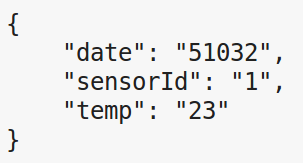
\includegraphics[width=0.4\linewidth]{graphics/JsonTemp}
\caption{Json\cite{json} string received from the WixelSensorService\label{fig:JsonTemp}}
\end{figure}
\subsubsection{Storage Service interface}
The storage service is an interface the developer needs to implement if a new way of
storing data is needed. The storage service interface has four virtual functions the developer needs to implement by inheriting from the StorageService class. The functions that needs implementation are the following:
\begin{itemize}
    \item \textbf{int save(String data)}
        \begin{itemize}
            \item Takes in data in String format and saves it to storage medium. 
                  Returns number of bytes saved, returns -1 if not enough space.
        \end{itemize}
    \item \textbf{String load()}
        \begin{itemize}
            \item Loads all data in memory and returns it in string format.
        \end{itemize}
    \item \textbf{int erase()}
        \begin{itemize}
            \item Erases all data from storage medium. Returns number of bytes
                  free after erase.
        \end{itemize}
    \item \textbf{bool isFreeSpcace(int dataSize)}
        \begin{itemize}
            \item Takes in size of data to be saved in bytes. Returns true if enough 
                  space is available, false if not.
        \end{itemize}
\end{itemize}
The storage service now implemented is the LocalStorageService. This service stores data 
to the Arduino's EEPROM. The Arduino Mega 2560 has 4096 bytes of 
EEPROM \cite{arduinoMega}. The LocalStorageService stores the data as series of Json 
strings. A typical use of the LocalStorageService is first to use the isFreeSpace() function to check if enough space is available for the data to be stored. If space is enough the save() function is used to save the data to the EEPROM. If space is not available the developer has to take some action like loading all existing data using the load() function, send the data to the HTTP server before using the erase() function to erase the EEPROM for new data. Pseudocode of the save(), load() and erase() functions can be seen in listings \ref{pseodoLocalStorageService}

\begin{lstlisting}[frame=single, label=pseodoLocalStorageService, caption={Pseudocode of LocalStorageService save(), load() and erase() functions}]
Function(save(data)):
    define iterator as 0
    define i = 0
    for i < EEPROM size:
        read byte i from EEPROM
        if byte i equals 0:
            break
        end if
        iterator = iterator + 1
        i = i + 1
    end for
    if not enough space for data:
        return -1
    else:
        define dataSize as 0
        define j as 0
        for j < data size in bytes:
            if iterator >= (EEPROM size -1):
                break
            end if
            write byte at index j in data to EEPROM address that equals iterator
            iterator = iterator + 1
            dataSize = dataSize +1
        end for
        write ',' to EEPROM address corresponding to iterator
        dataSize = dataSize + 1
        return dataSize
    end if
end Function(save(data))

Function(load):
    define data as string
    define i as 0
    define letter
    for i < EEPROM size:
        letter = byte at EEPROM address that equals i
        if letter equals 0:
            break
        end if
        append letter to data
    end for
    return data
end Function(load)

Function(erase):
    define counter as 0
    define i as 0
    for < EEPROM size:
        counter = counter + 1
        write 0 to EEPROM address that equals i
    end for
    if counter not equals EEPROM size:
        return -1
    else:
        return counter
    end if
Function(erase)
\end{lstlisting}

\subsubsection{Network Gateway interface}
The network gateway is an interface the developer needs to implement for each new way 
of communications with the outside world. The network gateway interface has five virtual 
functions the developer needs to implement by inheriting from the NetworkGateway class.
The functions needing implementation are the following:
\begin{itemize}
    \item \textbf{bool connectToNetwork()}
        \begin{itemize}
            \item Connects to network. Returns true if connected, false if not
                  connected.
        \end{itemize}
    \item \textbf{bool connected()}
        \begin{itemize}
            \item Checks if connected to network. Returns true if connected, false
                  if not connected.
        \end{itemize}
    \item \textbf{int sendData(String address, String data)}
        \begin{itemize}
            \item Sends given data to given address. Returns number of bytes sent, -1 if 
                  error sending data.
        \end{itemize}
    \item \textbf{String reciveData(String address)}
        \begin{itemize}
            \item Gets data from given address. Returns the data.
        \end{itemize}
     \item \textbf{long getTime()}
        \begin{itemize}
            \item Gets the current time/date from the network. Returns the time in UNIX time/date as long.
        \end{itemize}
\end{itemize}
The Network Gateways now implemented are the SmsGateway and the GprsGateway. The 
GprsGatway is based on code from Toby Fox\cite{tobek} and the SmsGateway utilizes the
SerialGSM library from Meir Michanie\cite{meirm}. Since SmsGateway is not yet fully
developed the GprsGateway will be described in detail here.

The GprsGateway sends gathered sensor data as Json objects via HTTP to a HTTP API
mentioned in chapter~\ref{HTTP-Server}. The GprsGateway uses AT commands\cite{ATcommands} to control the GPRS module. A typical use of the GprsGateway is first to check if the system is online by calling the connected() function. If the system is offline the 
connectToNetwork() function is called to connect to the GPRS network. When connected 
there are three functions to choose from; sendData(), receiveData and getTime. The 
sendData() function takes in the data as Json string and posts it to a given HTTP address
as REST\cite{rest} message. The receiveData() function receives data from a given HTTP
address. This can be used to update or change settings of the GeoLog. The getTime()function is used to get the current time from the network to sync the onboard clock.
Pseudocode for connectToNetwork() and sendData() functions can be seen in listings 
\ref{pseodoGprsGateway}

\begin{lstlisting}[frame=single, label=pseodoGprsGateway, caption={Pseudocode of GprsGateway connectToNetwork() and sendData() functions}]
Function(connectToNetwork):
    boot up GPRS module
    send "AT+CGATT=1" to the GPRS module
    wait for OK from the GPRS module
    if not received OK from GPRS module:
        return false
    end if
    send "AT+CGDCONT=1, IP, YOUR_APN" to the GPRS module
    wait for OK from the GPRS module
    if not received OK from GPRS module:
        return false
    end if
    send "AT+CGACT=1,1" to the GPRS module
    wait for OK from the GPRS module
    if not received OK from GPRS module:
        return false
    end if
    send "AT+SDATACONF=1, TCP, YOUR_SERVER_IP_ADDRESS, YOUR_SERVER_PORT_NUMBER"
    wait for OK from the GPRS module
    if not received OK from GPRS module:
        return false
    end if
    send "AT+SDATASTART=1,1" to the GPRS module
    wait for OK from the GPRS module
    if not received OK from GPRS module:
        return false
    end if
    return true
end Function(connectToNetwork)

Function(sendData(address, data)):
    define timeOut as desired timeout in milliseconds
    define data as "POST /geolog HTTP/1.1
                    Host: YOUR_HTTP_SERVER_ADDRESS
                    Content-Type: application/json
                    Content-Length: SIZE_OF_DATA_IN_BYTES

                    contents of data"
    if not connected to network:
        connectToNetwork()
    end if
    define inTime as time now in milliseconds
    while (time now in milliseconds - inTime) < timeOut:
        send "AT+SDATASTATUS=1" to the GPRS module
        get socketstatus from GPRS module
        if not received OK from GPRS module:
            return -1
        end if
        if socketstatus = "+SOCKSTATUS:  1,0,0104,0,0,0":
            wait for 1000 milliseconds
        else if socketstatus = "+SOCKSTATUS:  1,1,0102,0,0,0":
            break
        else:
            return -1
        end if
    end while
    define packetlength as size of data in bytes
    send "AT+SDATATSEND=1, packetLength\r" to the GPRS module
    if not received ">" from the GPRS module:
        return -1
    end if
    send data to the GPRS module
    send ctrl-z to the GPRS module
    if not received OK from GPRS module:
        return -1
    end if    
    define inTime as time now in milliseconds
    while (time now in milliseconds - inTime) < timeOut:
        send "AT+SDATASTATUS=1" to the GPRS module
        get socketstatus from GPRS module
        if socketstatus equals "+STCPD:1":
             get socketstatus from GPRS module
        end if
        if socketstatus equals "+STCPC:1":
            get socketstatus from GPRS module
        end if
        if not received OK from GPRS module:
            return -1
        end if
        if socketstatus not starts with "+SOCKSTATUS":
            return -1
        end if
        if socketstatus packet length equals packetlength:
            break
        else:
            wait for 1000 milliseconds
        end if
    end while
    send "AT+SDATASTATUS=0" to the GPRS module
    send "AT+SDATASTART=1,0" to the GPRS module
    if not received OK from GPRS module:
        return -1
    end if
    send "AT+CGATT=0" to the GPRS module
    if not received OK from GPRS module:
        return -1
    end if
    send "AAT+CGATT?" to the GPRS module
    set connected as false
    return 1
end Function(sendData)
\end{lstlisting}

\subsubsection{Main Runner}
The main runner is the .ino file, e.g. the Arduino sketch. It is up to the researcher
how it is set up although default setup is provided under the filename MainRunner.ino. 
Users are encouraged to modify the MainRunner to their needs. The MainRunner comes 
with number of helper functions and are as following:

\begin{itemize}
    \item \textbf{void collectData(int sensorId)}
        \begin{itemize}
            \item Used to collect data from sensor with given id. This function should
                  be modified if using other kind of sensor than provided.
        \end{itemize}
    \item \textbf{String parseDataToJson(int data, int sensorId)}
        \begin{itemize}
            \item Used to parse values from a given sensor and its id to Json object.
        \end{itemize}
    \item \textbf{String concatToJson(String data)}
        \begin{itemize}
            \item Makes a Json array of given data. Takes in data as stringified comma 
                  separated Json objects. 
        \end{itemize}
    \item \textbf{int sendToServer(String data)}
        \begin{itemize}
            \item Used to send given data to server. This might have to be modified
                  if using another kind of communications than provided.
        \end{itemize}
    \item \textbf{bool eraseRequest()}
        \begin{itemize}
            \item Used to erase the memory manually by pushing the erase button.
        \end{itemize}
    \item \textbf{bool manualSendRequest()}
        \begin{itemize}
            \item Used to send data to the server manually by pushing the manual send 
                  button
        \end{itemize}
\end{itemize}
A typical application of the MainRunner could be as shown in the pseudocode shown in listings \ref{pseodoMainRunner}

\begin{lstlisting}[frame=single, label=pseodoMainRunner, caption={Pseudocode of typical application of the MainRunner}]
define GSM_RESET_PIN as 22
define SAMPLE_DATA_FREQ as 300000 ms
define SEND_DATA_FREQ as 900000 ms
define TIME_OUT as 45000 ms
define MAX_TRIALS as 5
define ERASE_PIN as 50
define MANUAL_SEND_PIN as 51
define LED_PIN as 13
define sendRequest
define lastDataSample
define lastDataTransmit
define faildTransmits

Function(setup):
Set GSM_RESET pin as OUTPUT
Set ERASE pin as INPUT_PULLUP
Set MANUAL_SEND_PIN pin as INPUT_PULLUP
currentTime = current time
lastDataSample = current time
lastDataTransmit = current time
failedTransmits = 0
sendRequest = false
end Function(setup)

Function(loop):
if (current time - lastDataSample) > SAMPLE_DATA_FREQ or sendRequest equals true:
    collect data from sensor with id 1
    collect data from sensor with id 2
    collect data from sensor with id 3
    lastDataSample = current time
end if
if (current time - lastDataTransmit) > SAMPLE_DATA_FREQ or sendRequest equals true:
    load data from memory
    parse data to Json array
    send data to server
    if data was succesfully sent:
        erase memory
        lastDataTransmit = current time
        failedTransmits = 0
        sendRequest = false
    else if faildTransmits >= MAX_TRIALS:
        failedTransmits = 0
        lastDataTransmit = current time
        sendRequest = false
    else
        faildTransmits = faildTransmits + 1
    end if
end if
if manual erase button is pushed:
    erase memory
end if
if manual send data button is pushed:
    sendRequest = true
end if
end Function(loop)
\end{lstlisting}
\subsubsection{HTTP Server}\label{HTTP-Server}
\begin{figure}
\centering
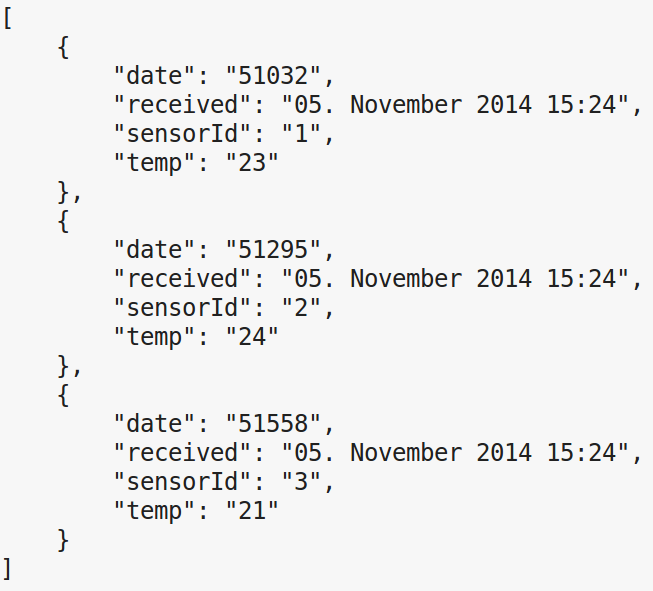
\includegraphics[width=0.6\linewidth]{graphics/JsonArray}
\caption{Json\cite{json} array received by the HTTP Server\label{fig:JsonArray}}
\end{figure}

The HTTP server designed for GeoLog is a Python Flask-Restful HTTP API
\cite{flask-restful}. The design was minimal and should only be able to
receive data from the GeoLog, store it and present it as a REST API and as more human
readable. The data arrives as a Json array as seen in figure \ref{fig:JsonArray}, the server parses the data and publishes it if the data is not corrupt. The human readable version is called GeoBlog. The code for the server is quite short and can be seen in the appendix under listings \ref{httpCode}.

\subsection{Safety}
The GeoLog is designed to withstand difficult weather conditions although care must be taken when setting it up. Before taking the GeoLog out to the elements make sure
every screw and fitting is tightened.\\
\textbf{Warning: Water or dirt might slip into the enclosure and damage the equipment if the sealing is not tight.}\\
\textbf{Warning: Do not use acid batteries cause they may leak and cause damage to your equipment.}\\
The software has been tested to meet the requirements stated in chapter 
\ref{requirements}. All modifications and changes are possible but can cause fail
in the equipment.
The GeoLog team is deprived from all liability for any kind of misuse of the 
equipment. The GeoLog is open source and the GeoLog Team welcomes contributors
at \url{https://github.com/GeoLogTeam/geolog}.



